% chktex-file 3 chktex-file 9 chktex-file 10 chktex-file 17 chktex-file 18 chktex-file 36 chktex-file 40
\section*{Exercise 1.2.}

\begin{enumerate}[label = (\alph*)]
    \item Show that a linear filter $\{a_j\}$ passes an arbitrary polynomial of degree $k$ without distortion, i.e.
    \[ m_t = \sum_{j} a_j m_{t-j} \]
    for all $k^{\mbox{th}}$ degree polynomials $m_t = c_0 + c_1 t + \cdots + c_k t^k$, if and only if
    \[ \begin{cases}
        \sum_{j} a_j = 1,\\
        \sum_{j}j^r a_j = 0, & \mbox{for }r = 1,\ldots, k.
    \end{cases} \]
    \item Show that the Spencer $15$-point moving average filter $\{a_j\}$ does not distort a cubic trend.
\end{enumerate}

\subsection*{Solution Part (a)}

$\boldsymbol{\implies}$ Let $\{a_j\}$ such that, for any $k^{\mbox{th}}$ degree polynomial $m_t = c_0 + c_1 t + \cdots + c_k t^k$
\[ m_t = \sum_{j} a_j m_{t-j}. \]
Let $c_0 = 1$ and $c_k = 0$ for $k > 0$ to see that
\[ m_t = 1 = \sum_{j} a_j \cdot 1. \]
Now, note that for $c_1 = 1$ and $c_k = 0$ for $k\neq 1$,
\[ m_0 = 0 = \sum_{j} a_j m_{-j} = -\sum_{j} a_j j \]
\[ \implies 0 = \sum_{j} a_j j \]
In general, for the polynomials with $c_{2i+1} = 1$ and $c_k = 0$ for $k \neq 2i+1$,
\[ m_0 = 0 = -\sum_{j} a_j j^{2i+1} \]
\[  \implies 0 = \sum_{j} a_j j^{2i+1} \]
and for $c_{2i} = 1$ and $c_k = 0$ for $k \neq 2i$,
\[ m_0 = 0 = \sum_{j} a_j (- j)^{2i} = \sum_{j} a_j j^{2i} \]
Therefore,
\[ \sum_{j}j^r a_j = 0,\hspace{1em} r \in \N^+. \]

$\boldsymbol{\impliedby}$ Let ${a_i}$ with $\sum_j a_j = 1$ and $\sum_j j^r a_j = 0$ for $ r = 1,\ldots, k$. Note that for any polynomial of degree $k$ $m_t$,
\[ \everymath{\displaystyle}
\arraycolsep=1.8pt\def\arraystretch{2.5}
\begin{array}{rcl}
    \sum_{j} a_j m_{-j}
    & = & \sum_{j} a_j \sum_{r = 0}^k c_r (-j)^r\\
    & = & \sum_{r = 0}^{k} c_r (-1)^r \underbrace{\sum_{j} a_j j^r }_{r \neq 0 \implies 0} = c_0 = m_0
\end{array} \]
Similarly, for the $n$-th derivative of $m_t$,
\[ \everymath{\displaystyle}
\arraycolsep=1.8pt\def\arraystretch{2.5}
\begin{array}{rcl}
    \sum_{j} a_j m^{(n)}_{-j}
    & = & \sum_{j} a_j \sum_{r = 0}^k c_r \frac{r!}{(r-n)!} (-j)^{r-n}\\
    & = & \sum_{r = 0}^{k} c_r \frac{(-1)^{r-n} r!}{(r-n)!} \underbrace{\sum_{j} a_j j^{r-n} }_{r \neq n \implies 0} = n! c_n = m^{(n)}_0
\end{array}
\]
Finally, using Taylor's theorem
\[ \everymath{\displaystyle}
\arraycolsep=1.8pt\def\arraystretch{2.5}
\begin{array}{rcl}
    m_t & = & \sum_{n = 0}^{k} \frac{m^{(n)}_0}{n!} t^n\\
    & = & \sum_{n = 0}^k \sum_{j} a_j \sum_{r = 0}^k c_r \frac{r!}{n! (n-r)!} t^n (-j)^{n-r}\\
    & = & \sum_{j} \sum_{n = 0}^k a_j \sum_{r = 0}^k c_r \frac{r!}{n! (n-r)!} t^n (-j)^{n-r}\\
    \mbox{\tiny{(Cauchy-Product)}} & = & \sum_j a_j \sum_{r = 0}^{k} c_r \sum_{n = 0}^r \frac{r!}{n! (n-r)!} t^n (-j)^{n-r}\\
    \mbox{\tiny{(Binomial-Theorem)}} & = & \sum_j a_j \sum_{r = 0}^{k} c_r (t-j)^r\\
    & = & \sum_{j} a_j m_{t-j}.
\end{array} \]

\subsection*{Solution Part (b)}
Using the lemma we proved in the previous part,
\[ \sum_{j = -7}^{7} a_j = \frac{1}{320}(-3-6-5+3+21+46+67+74+67+46+21+3-5-6-3) = \frac{320}{320}. \]

\begin{figure}[H]
    \centering
    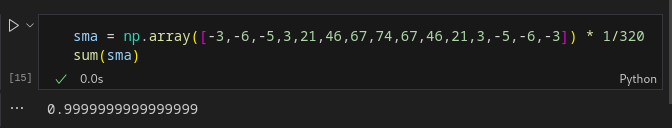
\includegraphics[width=0.85\textwidth]{../pictures/hw1ex1.2.1.png}
\end{figure}

\[ \sum_{j = -7}^{7} a_j j^r = 0\]

\begin{figure}[H]
    \centering
    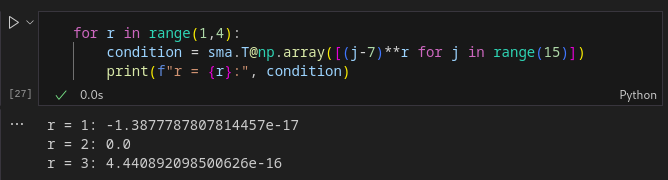
\includegraphics[width=0.85\textwidth]{../pictures/hw1ex1.2.2.png}
\end{figure}